\documentclass[a4paper,12pt]{article}
\usepackage{color}
\usepackage{graphicx}
\begin{document}

\title{\textbf{Working With Ngspice And Geda Schematic}}
\author{Nazrul}
\date{\today}
\maketitle

\pagenumbering{roman}
\tableofcontents
\newpage
\pagenumbering{arabic}

\section{Introduction}
The purpose of this document is to show how to use ngspice and geda in parallel to analyze circuits and produce desired outputs.

\section{Installation}
Lets install both the requiresd software in the system before we proceed. Since the project has been done on a linux system, It will be assumed that the user is operationg a linux os, prefrebaly Ubuntu.

Type in this command and follow along the terminal to install the packages.

{\color{green}sudo apt install ngspice}

{\color{green}sudo apt install geda}

\textit{\color{red}Please note that this commands has to be run as a rrot user to install it properly!}

\newpage

\section{Drawing the Schematic}

The first part of the method is to have a working schematic. To achive this open gschem.\textbf{Draw this schematic and add all the values as shown in figure.}

\begin{figure}[h!]
\centering
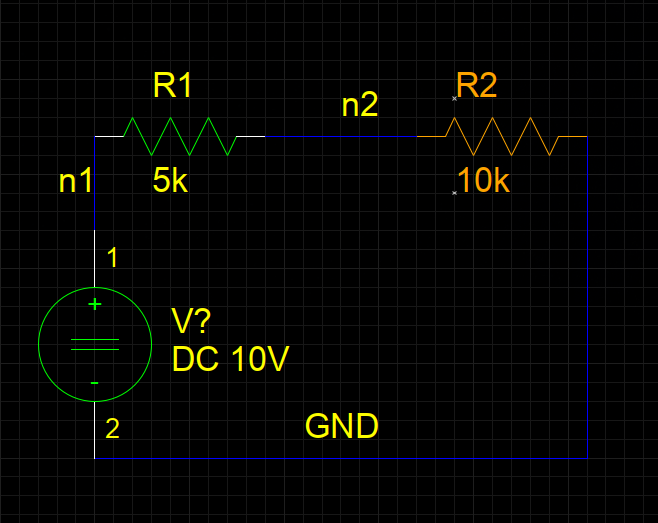
\includegraphics[width=1\textwidth]{Schematic.png}
\caption{Schematic}
\end{figure}

\newpage

\section{Generating the netlist!}
Follow the commands in the terminal from the image below!

\begin{figure}[h!]
\centering
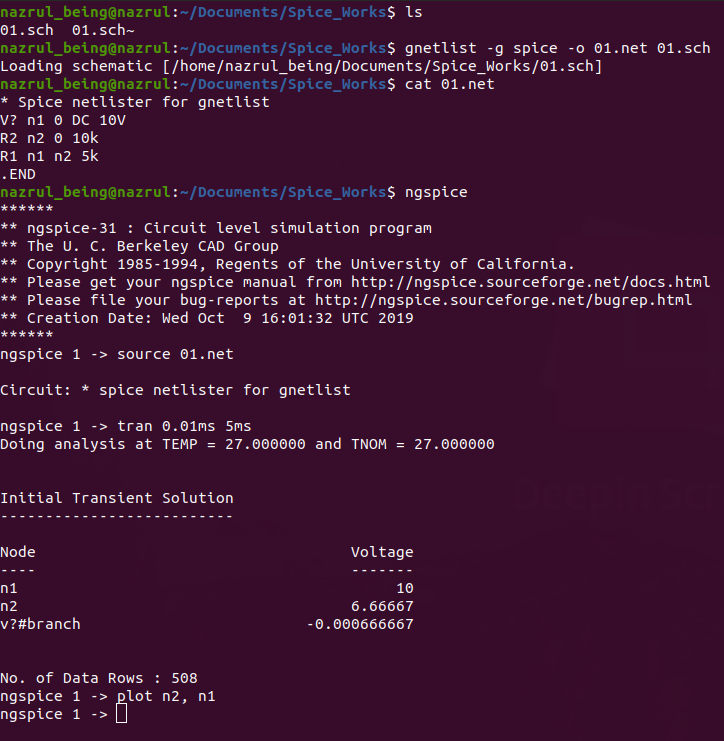
\includegraphics[width=1\textwidth]{Terminal.png}
\caption{Schematic}
\end{figure}

under the part Initial Transient Solution in the figure we can see that we have some values. We will plot the graph using this values to better visualize what is happening in the circuit.


\section{Plot}
After performing all commands described in the previous section. we can see we obtain a graph similar to this.

\begin{figure}[h!]
\centering
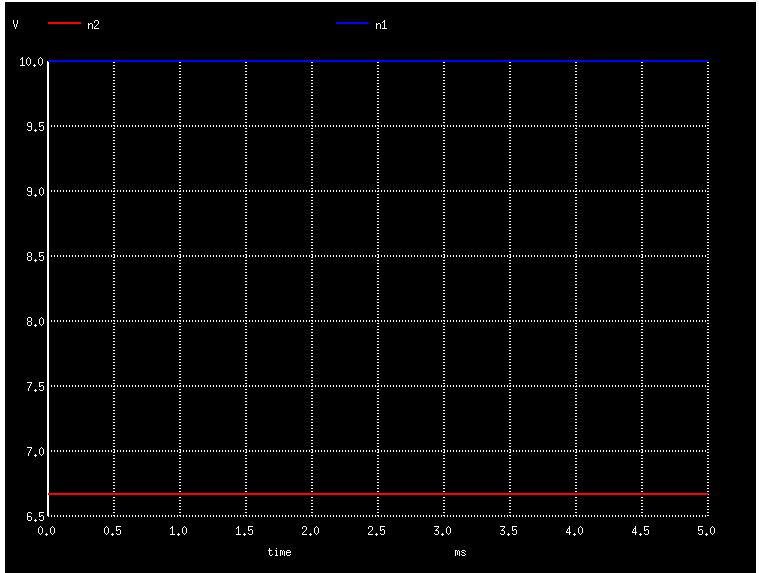
\includegraphics[width=1\textwidth]{011.png}
\caption{Schematic}
\end{figure}

\section{Result}
As we can see that the circuit is a simple voltage divider. but using this form of analysis gives us much better understanding of whats happening in the circuit. and at the same time allows for solving the curcuit with much less effort and accuretly.

\newpage
\centering
\textbf{Thankyou for Reading!}

\end{document}
